\documentclass[journal,12pt,twocolumn]{IEEEtran}
\usepackage{cite}
\usepackage{amsmath,amssymb,amsfonts,amsthm}
\usepackage{algorithmic}
\usepackage{graphicx}
\usepackage{textcomp}
\usepackage{xcolor}
\usepackage{txfonts}
\usepackage{listings}
\usepackage{enumitem}
\usepackage{mathtools}
\usepackage{gensymb}
\usepackage{comment}
\usepackage[breaklinks=true]{hyperref}
\usepackage{tkz-euclide} 
\usepackage{listings}
\usepackage{gvv}                                        
\def\inputGnumericTable{}                                 
\usepackage[latin1]{inputenc}                                
\usepackage{color}                                            
\usepackage{array}                                            
\usepackage{longtable}                                       
\usepackage{calc}                                             
\usepackage{multirow}                                         
\usepackage{hhline}                                           
\usepackage{ifthen}                                           
\usepackage{lscape}
\usepackage{caption}
\usepackage{subfigure}

% Define \phase command
\newcommand{\phase}[1]{\text{arg}\left(#1\right)}

\newtheorem{theorem}{Theorem}[section]
\newtheorem{problem}{Problem}
\newtheorem{proposition}{Proposition}[section]
\newtheorem{lemma}{Lemma}[section]
\newtheorem{corollary}[theorem]{Corollary}
\newtheorem{example}{Example}[section]
\newtheorem{definition}[problem]{Definition}
\newcommand{\BEQA}{\begin{eqnarray}}
\newcommand{\EEQA}{\end{eqnarray}}
\newcommand{\system}[1]{\stackrel{#1}{\rightarrow}}
\newcommand{\define}{\stackrel{\triangle}{=}}
\theoremstyle{remark}
\newtheorem{rem}{Remark}

\begin{document}

\bibliographystyle{IEEEtran}
\vspace{3cm}

\title{Gate.in.21}
\author{EE22BTECH11008 - Annapureddy Siva Meenakshi$^{*}$}
\maketitle
\bigskip

\renewcommand{\thefigure}{\theenumi}
\renewcommand{\thetable}{\theenumi}
Q: A system has transfer function
\[\frac{Y(s)}{X(s)}=\frac {s-\pi}{s+\pi}\]
let $u(t)$ be the unit step function. The input $x(t)$ that results in a steady-state output $y(t)=\sin(\pi t)$ is \underline{\quad}.
\solution

\begin{figure}[htb]
  \centering
  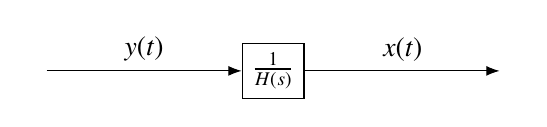
\begin{tikzpicture}[auto, node distance=4cm,>={Latex}]
  % Define blocks
  \node (input) at (0,0) {};
  \node [draw, rectangle] (H) at (3,0) {$\frac{1}{H(s)}$}; 
  \node (output) at (6,0) {};

  % Connect blocks with right arrows
  \draw [->] (input) -- node[midway, above] {$y(t)$} (H);
  \draw [->] (H) -- node[midway, above] {$x(t)$} (output);
\end{tikzpicture}

  \captionsetup{justification=centering, singlelinecheck=off}
  \caption{Block diagram of the inverse system}
  \label{fig:in_21_f1}
\end{figure}

\begin{figure}[htb]
  \centering
  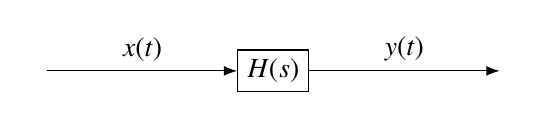
\begin{tikzpicture}[auto, node distance=4cm,>={Latex}]
  % Define blocks
  \node (input) at (0,0) {};
  \node [draw, rectangle] (H) at (3,0) {$H(s)$};
  \node (output) at (6,0) {};

  % Connect blocks with right arrows
  \draw [->] (input) -- node[midway, above] {$x(t)$} (H);
  \draw [->] (H) -- node[midway, above] {$y(t)$} (output);
\end{tikzpicture}

  \captionsetup{justification=centering, singlelinecheck=off}
  \caption{Block diagram of the system}
  \label{fig:in_21_f2}
\end{figure}

\begin{table}[!ht]
    \centering
        \begin{tabular}{|c|c|c|} 
    \hline
    \textbf{Variable} & \textbf{Description} & \textbf{Value} \\
    \hline
    $x(t)$ & input function & none \\
    \hline
    $y(t)$ & output function & $\sin(\pi t)$ \\
    \hline
    $H(s)$ & Transfer-function & $\frac{s-\pi}{s+\pi}$ \\
    \hline
\end{tabular}

    \caption{Input parameters}
    \label{tab:in_21_t1}
\end{table}

\begin{equation}
    H(s) = \frac{s - \pi}{s + \pi} 
\end{equation}
from ~\figref{fig:in_21_f1}
\begin{equation}
	\frac{1}{H(s)} = \frac{s + \pi}{s - \pi}
\end{equation}
Converting transfer function to frequency response, we get
\begin{equation}
    \frac{1}{H(j\omega)}=\frac{j\omega+\pi}{j\omega-\pi}
\end{equation}
from ~\tabref{tab:in_21_t1} $\omega=\pi$
\begin{equation}
   \frac{1}{H(j\pi)} = \frac{j + 1}{j - 1} = -j = e^{-j\frac{\pi}{2}}\label{eq:in.21.4} 
\end{equation}
from ~\eqref{eq:in.21.4} 
\begin{equation}
	\abs{\frac{1}{H(j\pi)}}=1 \quad \text{and} \quad \phase{\frac{1}{H(j\pi)}} = -90^\circ
\end{equation}
\begin{equation}
    y(t) = \sin(\pi t) \label{eq:in.21.6}
\end{equation}

\begin{align}
  \sin(\pi t)&\system{\frac{1}{H(j\omega)}}\abs{\frac{1}{H(j\omega)}}\sin\left(\pi t  + \phase{\frac{1}{H(j\omega)}}\right)\label{eq:in.21.8}
\end{align}

Therefore, by ~\eqref{eq:in.21.6} and ~\eqref{eq:in.21.8}, we get
\begin{equation}
    x(t)=\sin\left(\pi t -\frac{\pi}{2}\right)
\end{equation}

\begin{figure}[h]
  \centering
  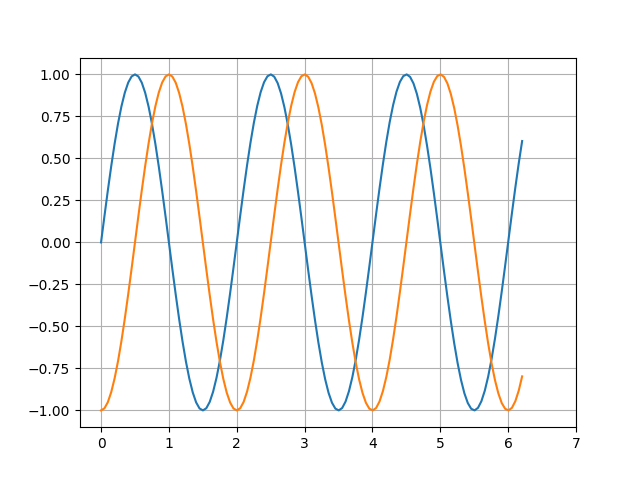
\includegraphics[width=\columnwidth]{./figs/figure3.png} 
  \captionsetup{justification=centering}
  \caption{Plot of $x(t)$ and $y(t)$ taken from Python}
  \label{fig:in.21.f3}
\end{figure}

\begin{figure}[h]
  \centering

  \subfigure[Amplitude of $\frac{1}{H(j\omega)}$]{
    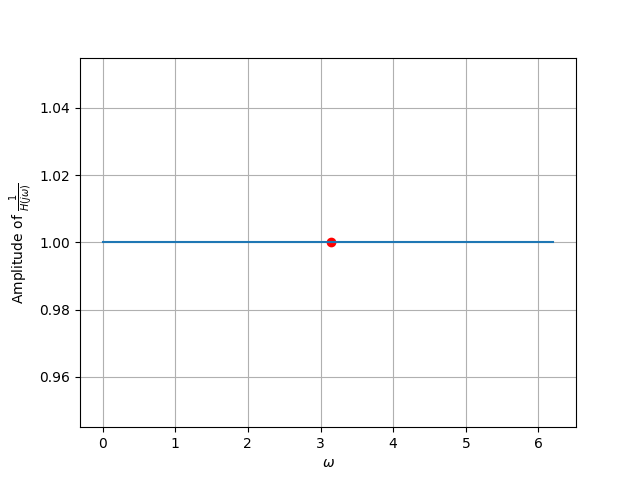
\includegraphics[width=0.45\linewidth]{./figs/figure1.png}
    \label{fig:in.21.subfig.1}
  }
  \hfill
  \subfigure[Phase of $\frac{1}{H(j\omega)}$]{
    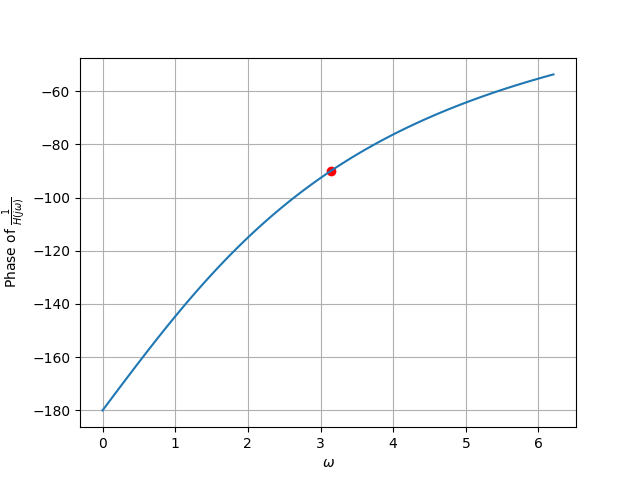
\includegraphics[width=0.45\linewidth]{./figs/figure2.png}
    \label{fig:in.21.subfig.2}
  }
  \caption{Amplitude and Phase of $\frac{1}{H(j\omega)}$}
  \label{fig:in.21.subfig}
\end{figure}

\end{document}

